\begin{proof}(теоремы Дирихле).
	При $\displaystyle \Re(s)>1 \ -\frac{L'(s,\,\chi)}{L(s,\,\chi)} = \sum\limits_{n=1}^\infty \frac{\Lambda(n)\chi(n)}{n^s}$.\\
	Пусть далее $s=\sigma \in \mathbb{R}, \, s>1$. $\Lambda(n) = 
	\begin{cases}
		\ln p, & n=p^k,\,k\geq1,\\
		0, & \text{иначе.}
	\end{cases}$
	Тогда 
	$$-\frac{L'(s,\,\chi)}{L(s,\,\chi)} = \sum\limits_p \frac{\ln p \chi(p)}{p^s} + \sum\limits_p \sum\limits_{k=2}^\infty \frac{\ln p \cdot \chi\left( p^k \right)}{p^{ks}}$$ (первое слагаемое для $n=p$, второе -- для $n=p^k$). Покажем, что второе слагаемое ограничено константой, не зависящей от $s$ при $s>1$:
	$$\left| \sum\limits_p \sum\limits_{k=2}^\infty \frac{\ln p \cdot \chi\left( p^k \right)}{p^{ks}} \right| \leq \sum\limits_p \sum\limits_{k=2}^\infty \frac{\ln p}{p^{ks}} = \sum\limits_p \ln p \frac{1/p^2}{1-1/p} \leq 2\sum\limits_p \frac{\ln p}{p^2} < 2\sum\limits_n \frac{\ln n}{n^2} < \infty.$$
	Итак, для любого характера $\chi$ по модулю $m$:
	$$\sum\limits_p \frac{\chi(p)\ln p}{p^s} = -\frac{L'(s,\,\chi)}{L(s,\,\chi)} + O(1). \qquad \qquad (\ast)$$
	Поскольку $(l, m) =1$, то $\exists v \in \mathbb{Z}: \ vl \equiv 1 \ (\mathrm{mod} \ m)$ (т.е. обратный). 
	Домножим $(\ast)$ на $\chi(v)$ и просуммируем по всем характерам:
	$$\sum\limits_p \frac{\ln p}{p^s} \sum\limits_\chi \chi(pv) = -\sum\limits_\chi \chi(v)\frac{L'(s,\,\chi)}{L(s,\,\chi)} + O(1),$$
	$$\sum\limits_\chi \chi(pv) = 
	\begin{cases}
		0, & pv \not\equiv 1 \ (\mathrm{mod} \ m),\\
		\phi(m), & pv \equiv \ (\mathrm{mod} \ m).
	\end{cases}$$
	Но $pv \equiv 1 \ (\mathrm{mod} \ m)$, следовательно, $p \equiv l \ (\mathrm{mod} \ m)$ т.к. $pl \equiv 1 \ (\mathrm{mod} \ m)$. Значит,
	$$\sum\limits_{p \equiv l \ (\mathrm{mod} \ m)} \frac{\ln p}{p^s} = -\frac{1}{\phi(m)} \sum\limits_\chi \chi(v)\frac{L'(s,\,\chi)}{L(s,\,\chi)} + O(1).$$
	Перейдём к пределу при $s \to 1+$. Если $p \equiv l \ (\mathrm{mod} \ m)$ конечное количество, то слева предел конечен. Докажем, что правая часть стремится к бесконечности (т.е в левой части бесконечное число слагаемых):\\
	При $\displaystyle \chi \ne \chi_0 \ \ \frac{L'(s,\,\chi)}{L(s,\,\chi)} = O(1)$ при $s \to 1+$.\\
	При $\displaystyle \chi = \chi_0 \ \ L(s,\,\chi) = \frac{f(s)}{s-1}$, где $f(s)$ аналитична в $1$ и $f(1) \ne 0$.\\
	Значит,
	$$\frac{L'(s,\,\chi_0)}{L(s,\,\chi_0)} = -\frac{1}{s-1} + \frac{f'(s)}{f(s)} = -\frac{1}{s-1} + O(1) \xrightarrow{\text{при } s\to1+} \infty.$$
	То есть мы показали, что правая часть стремится к бесконечности при $s \to 1+$. Следовательно,
	$$\sum\limits_{p \equiv l \ (\mathrm{mod} \ m)} \frac{\ln p}{p^s} = \frac{1}{\phi(m)(s-1)} + O(1).$$
\end{proof}
Из последнего равенства можно, в частности, получить, что $\displaystyle \sum\limits_p \frac{\ln p}{p^s} = \frac{1}{s-1} + O(1)$.\\

\newpage

\section{Диофантовы приближения}
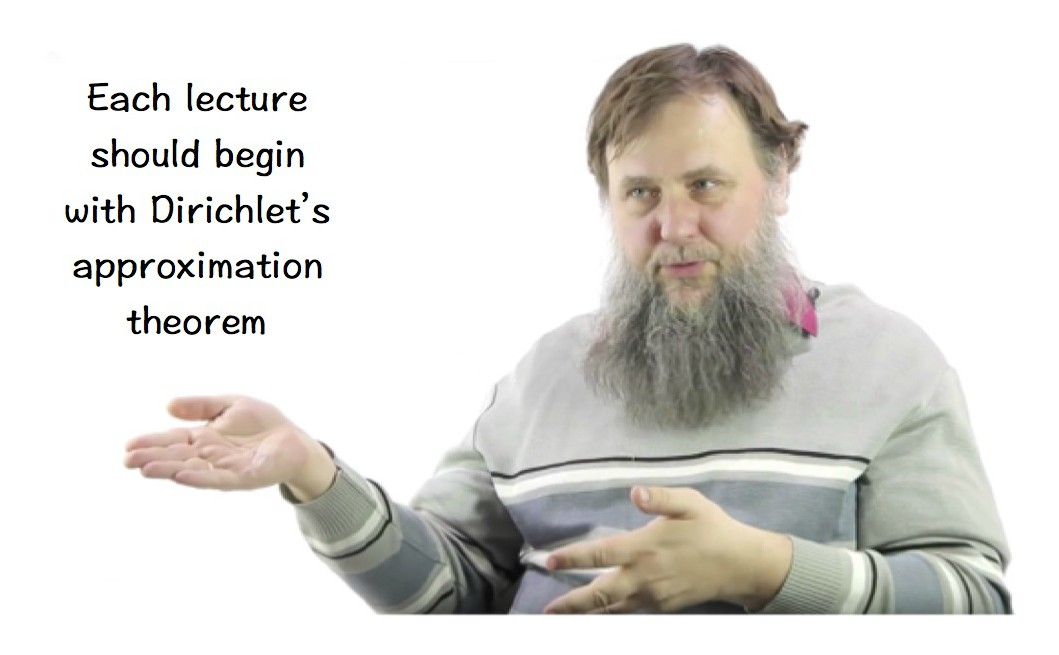
\includegraphics[width=\textwidth]{moschevitin}~\\

\subsection{Основные сведения}
	Пусть $\theta \in \mathbb{R}$. Насколько маленькой можно сделать разность $\lvert \theta - \frac{p}{q} \rvert$ так, чтобы $\lvert \theta - \frac{p}{q} \rvert < f(a)$ ($p$ и $q$ -- не простые).\\
	Характеристика $\theta$: насколько хорошо она приближается $\frac{p}{q}$. Мы знаем, что существуют нерациональные числа ($\sqrt{2}, \, \sqrt{3},\dots$). Легко доказать, что корни многочленов с целыми коэффициентами (алгебраические числа) не будут рациональными. Например, у многочлена $x^2 - x -1 =0$ корень $\phi = \frac{1+\sqrt{5}}{2}$, а у него корни имею вид $\frac{\text{делитель } -1}{\text{делитель} 1} \in \{ \pm 1 \}$ -- $\pm 1$ оба не корни.\\
	А вдруг все числа алгебраические? Нет, алгебраических чисел счётное количество. Это доказал Лиувилль через теорию приближений: он показал, что алгебраические числа не могут приближаться "слишком хорошо". Т.е. для алгебраических чисел не найдётся такой $f$, для которой будет бесконечно много решений.\\

\begin{statement}
	Если $\displaystyle \theta = \frac{a}{b} \in \mathbb{R}$, то $\displaystyle \forall \frac{p}{q} \in \mathbb{Q} \backslash \{ 0 \}$ такая, что 
	$\displaystyle \left| \theta - \frac{p}{q} \right| > \frac{1/b}{q}$.
\end{statement}
\begin{proof}
	$\displaystyle \left| \frac{a}{b} - \frac{p}{q} \right| = \frac{|aq - bp|}{bq} \geq \frac{1}{bq}$, т.к. $|aq-bp| \in \mathbb{Z} \ \ne 0$.
\end{proof}

\begin{theorem}[Дирихле о приближении] \label{l8_thmDir}~\\
	Пусть $\theta \in \mathbb{R}, \, T \in \mathbb{N}$. Тогда 
	$\displaystyle \exists \frac{p}{q} \in \mathbb{Q}: \ \left| \theta - \frac{p}{q} \right| < \frac{1}{qT}, \ 1 \leq q \leq T$.
\end{theorem}
\begin{proof}~\\
	Хотим: $\displaystyle |q\theta - p| < \frac{1}{T}$. Можно считать, что $\theta \in [0, \, 1)$, потом просто прибавить целую часть.\\
	Рассмотрим числа $\{ n\theta \}, \ n = 0,1,\dots,T$. Разобьём отрезок $[0, \, 1]$ на полуинтервалы 
	$\displaystyle \left[ \frac{k}{T}, \, \frac{k+1}{T} \right), \, k=0,1,\dots,T-1$ (т.е на $T$ равных). По принципу Дирихле 
	$\displaystyle \exists n_1,n_2: \ \left( n_1 - n_2 \right)\theta - \left( \left[n_1\theta\right]-\left[n_2\theta\right] \right) < \frac{1}{T}$. 
	Остаётся положить $q = n_1-n_2, \, p = \left[ n_1\theta \right] - \left[ n_2\theta \right]$; $q \geq 1, \, q \leq T$ (т.е. $n_1,\,n_2 \leq T$).
\end{proof}

\begin{corollary}
	Если $\theta \in \mathbb{R} \backslash \mathbb{Q}$, то неравенство 
	$\displaystyle \lvert \theta - \frac{p}{q} \rvert < \frac{1}{q^2}$ имеет бесконечно много решений в $\frac{p}{q} \in \mathbb{Q}$.
\end{corollary}
\begin{proof}
	От противного: пусть $\displaystyle \frac{p_1}{q_1},\dots,\frac{p_k}{q_k}$ -- все решения $\displaystyle \left| \theta - \frac{p}{q} \right| < \frac{1}{q^2}$. Положим $\displaystyle \delta = \min\limits_i \left| \theta - \frac{p_i}{q_i} \right| > 0, \, T = \lceil \frac{1}{\delta} \rceil$ (любое $\displaystyle T > \frac{1}{\delta}$). По теореме \ref{l8_thmDir} Дирихле $\displaystyle \exists \frac{p}{q}, \ q \leq T: \ \left| \theta - \frac{p}{q} \right| < \frac{1}{qT} \leq \frac{1}{q^2}$. Т.е. $\displaystyle \frac{p}{q}$ должно быть среди $\displaystyle \frac{p_i}{q_i}$. Но $\displaystyle \left| \theta - \frac{p}{q} \right| < \frac{1}{qT} < \frac{\delta}{q} \leq \delta$, т.е. оно ближе, чем наименьшее $\delta$. Противоречие.
\end{proof}

Мера иррациональности числа $\displaystyle \theta = \sup\limits_s : \ \{ \left| \theta - \frac{p}{q} \right| < \frac{1}{q^s} \text{ имеет бесконечно много решений } \frac{p}{q} \}$.

В качестве $\displaystyle \frac{p}{q}$ можно брать подходящие дроби в разложении $\theta$ в цепную дробь.